\documentclass[main.tex]{subfiles}

\begin{document}

\chapter{Technological Background} \label{section:back}


\section{Parallel Computing}

Traditional computer programs are written in a sequential manner. It is natural to think of an algorithm as a sequence of steps that can be serially performed to achieve a final result. This has actually been the most common programming paradigm since the early days of computing, and it synergizes well with single processor machines. Optimizations related to instruction-level parallelism, such as out-of-order execution, pipelining, branch prediction or superscalarity, were mostly handled by the compiler or the hardware itself, and transparent to the programmer. Vector processing was also a key performance factor, allowing the same instruction to be applied to a vector of data simultaneously, rather than one at a time (commonly referred to as \ac{SIMD}).

But in the beginning of the \rom{21} century, the development of computational chips shifted from a single faster core perspective, to a multi core one. The evolution of single-core processors was already reaching its peak, and was slowing down due to the increasing difficulty in reducing transistor size or increasing clock frequencies, while introducing or aggravating other problems, such as heat dissipation, which becomes harder with the increased complexity of a chip. The solution was to move a multi-core perspective, coupling more cores in the same chip, to share the workload and allow overall computational capabilities to keep evolving.

This has allowed hardware development to keep in conformance with Moore's Law\footnote{A prediction by Gordon Moore, stating that approximately every two years, the number of transistors in a computer chip would double} \cite{schaller1997moore}. And while it was a necessary step from a hardware's perspective, this has important implications in software development. In order for an application to take advantage of multi-core technology, it needs to be broken into smaller tasks, that can be independently executed, or with some level of synchronization and communication between them. Writing parallel algorithms requires an adaptation to this new paradigm, as a sequential line of execution does not provide efficient results in platforms that support parallel execution of several threads or processes.




\section{The \gpu as a Computing Accelerator}

With the increasing demand for highly data-parallel algorithms, and the growing amount of data to process, hardware development started shifting towards the goal of solving that problem. Initially, that started with the increased support for vector instructions in common \acsp{CPU}, and the \acs{SIMD} model. This allowed a single instruction to operate on a set of elements at once, effectively achieving a kind of parallelism which was extremely useful with highly data-parallel applications. Modern Intel processors, starting with the Sandy Bridge family, already support \ac{AVX}, an extension to the \textit{x86} instruction set allowing \acs{SIMD} instructions capable of handling 256 bits registers. This extension also introduces three-operand \acs{SIMD} instructions that allow more general $c = a + b$ operations to be handled with a single instruction, in addition to the previous instructions which only allowed two operands ($a = a + b$).

A similar and more flexible model is the usage of a single instruction across multiple threads running concurrently, called \ac{SIMT}. This is the programming model behind \gpus, which gradually started to gain more attention for their general purpose computing capabilities. Although the hardware of a \gpus is still tightly coupled with graphics processing and rendering, there have also been several advances in their usage as \gpgpus.


%%%%%%%%%%%%%%%%%%%%%%%%%%%%%%%%%%%%%%%
\subsection{Fermi Architecture}

The Fermi architecture was an important milestone of \gpus technology, as it was one of the first generations target directly towards \gpgpu and high performance computing, rather than just graphics rendering. The first Fermi devices were released in 2010, and were the first NVidia products to include support for double precision floating point number, which was an important feature for high performance computing to provide more accurate results. Fermi devices also included a GDDR5 memory controller with support for \ac{DMA} through the \acs{PCIe} bus, and up to 16 \acf{SM}, for a total of up to 512 \acs{CUDA} Cores.

Each \sm can access a total of 64KB of private memory, which can be configured to be split between shared memory and L1 cache, although configuration was restricted to either 48KB + 16KB or 16KB + 48KB. This provided some flexibility to the devices, since some problems would benefit more from the extra shared memory and not so much from cache, and vice-versa.

Additionally, all \acsp{SM} share a common 768KB L2 cache, and a final level of global memory, external to the chip, that can go up to 6GB of GDDR5, with a bandwidth of 192.6 GB/s in the Tesla C2070 \cite{NVIDIA:fermi}.

\begin{figure}[!htp]
  \centering
  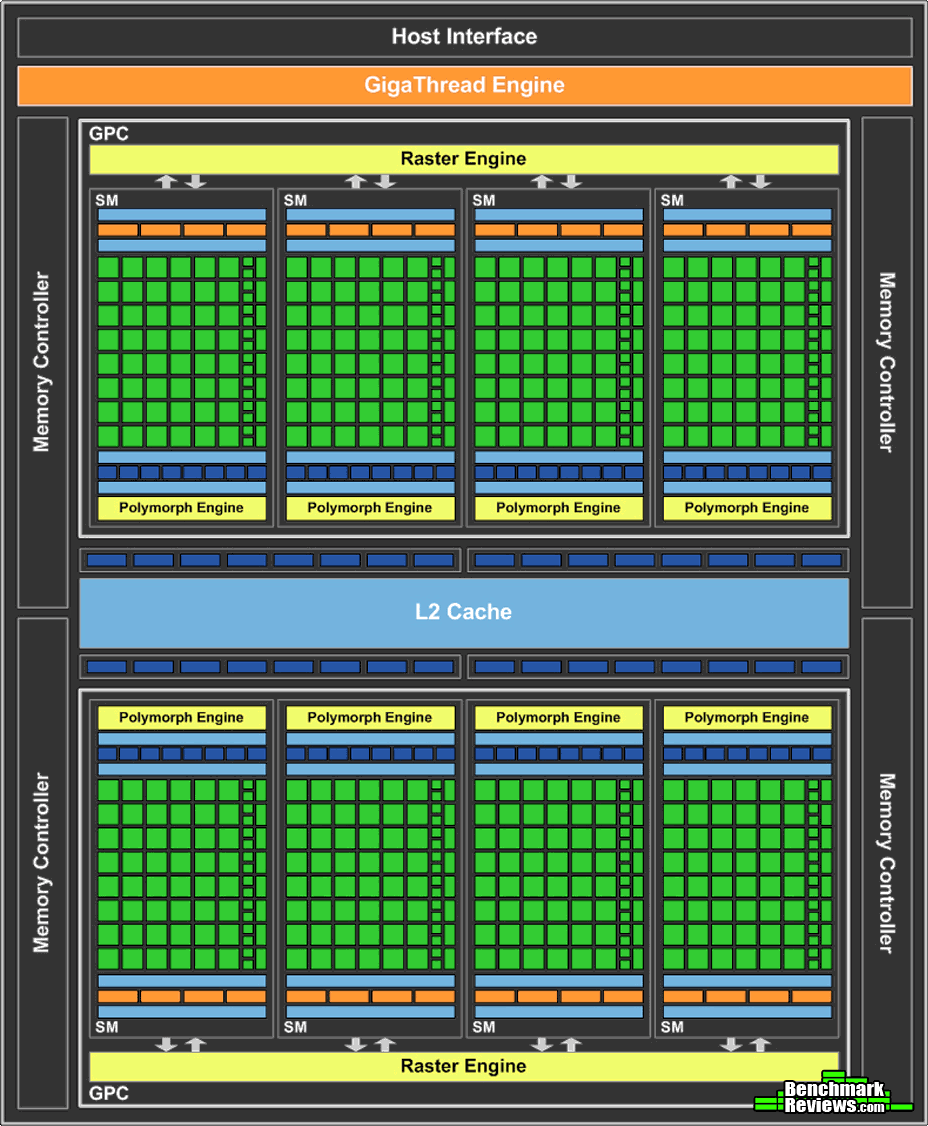
\includegraphics[width=0.6\textwidth]{arch_fermi}
  \caption{Overview of the Fermi architecture \label{fig:fermi}}
\end{figure}

This architecture is backed by a hardware-based thread scheduler, located within each \acs{SM}, that attempt to feed the execution unit with threads grouped in blocks of 32, or \textit{warps}. All threads within a warp are considered to be independent from each other, so there is no need for dependency checking. Any thread that is waiting for memory accesses to be finished will remain unscheduled until the required data is available. Since the scheduling is made directly via hardware, the switch between threads is nearly free, at least when compared with thread scheduling on a \acs{CPU}. As a result, this strategy works better when the total amount of threads competing for resources is much higher than the amount of execution units, allowing for the latency of memory accesses to be hidden away by instantly scheduling a different \textit{warp}, effectively hiding memory latency while still keeping execution units busy. This is very different from \acs{CPU} scheduling policies, where switching between threads requires a context switch, which takes considerably longer, making that approach not as feasible as for a \gpus.



%%%%%%%%%%%%%%%%%%%%%%%%%%%%%%%%%%%%%%%%
\subsection{Kepler Architecture}

The follow-up generation to Fermi is in many ways similar to its predecessor. One of the most notorious change is the increase in the total amount of available CUDA cores, capable of going up to 2880 in high-end devices, due to the redesign of the \acl{SM}, now called \smx, each one with 192 \cuda Cores, although working at lower frequencies than before, due to the removal of shader frequency, a compromise to make room for the extra \cuda Cores. The entire chip now works based on the core frequency. Overall, individual core efficiency is lowered, but the global system becomes more efficient.

\begin{figure}
  \centering
  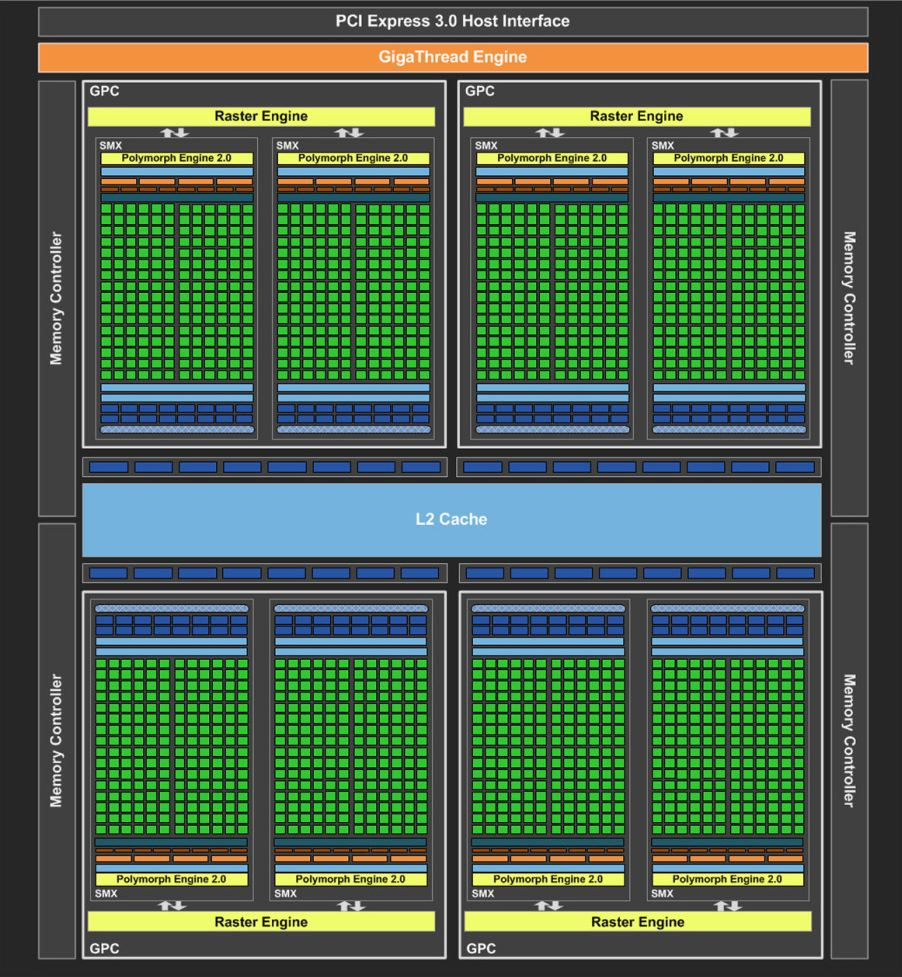
\includegraphics[width=0.6\textwidth]{arch_kepler}
  \caption{Overview of the Kepler architecture \label{fig:kepler}}
\end{figure}

The memory hierarchy was also upgraded over the previous generations, with the maximum amount of registers per thread going from 63 to 255, the addition of an extra 48KB L1 read-only cache, while still maintaining the original L1 cache (which now also allows a configuration of 32KB shared + 32KB cache), and L2 cache going up to a maximum of 1.5MB with increased bandwidth. Memory reads have been upgraded to allow for 256-bit blocks to be read, as opposed to 128-bit in Fermi \cite{NVIDIA:kepler}.

The programming model has been extended with the addition of dynamic parallelism, allowing \acs{CUDA} thread to spawn new threads, a feature not possible with previous versions. This is an important feature for irregular algorithms, such as photon mapping. It is also possible to invoke multiple kernels for a single \gpu, transparently dividing them between the available \smxs.


\itodo{Xeon Phi}




\section{Heterogeneous Platforms}

Initial programming methodologies for \hetplats consists mostly on programming the main application structure to a regular \cpu core, and offload some of the heavily data-parallel work to an accelerator, usually a \gpu. This often is coupled with manual testing to assert whether or not executing the task on the accelerator device, along with the required memory transactions, are actually beneficial to the overall performance.
With the increased acceptance of accelerators as co-processors, development efforts have been made towards making this development process much easier, and thus produce more, and better applications.

To address this problem, several frameworks have been proposed in the last years. These frameworks are usually targeted specifically at \acp{HetPlat}, and are designed with a focus on their specific scheduling issues, which are considered a key issue. These frameworks include StartPU \cite{augonnet2011starpu}, Harmony \cite{diamos2008harmony}, and GAMA. \todo{a cena coreana que o zuca tinha dito a uns tempos}

These frameworks aim to provide a bridge for programmers do develop applications suited to \hetplat, by addressing problems such as memory management or the scheduling of multiple tasks issued for execution. Most of them however, provide mechanisms suited mostly for regular applications. When dealing with irregular applications, problems like scheduling become even more difficult, in particular because execution times and memory usage patterns are less predictable. This directly affects the decisions of the scheduler, and as such must be taken into account by the performance model employed by the framework. Irregular applications are one of the targets of the \gama framework, which will be object of study throughout this dissertation, through the implementation of an irregular algorithm as a case study.

\subsection{A note on debugging}

It is hard enough to debug multi-threaded \cpu applications, and the addition of an extra device, with a different architecture, and possibly different mechanisms to handle debugging, introduces yet another layer of complexity to the development process. Conceptually, it is much harder for the programmer to keep track of the debugging process, since there is not as much control over what is happening. For instance, unless threads are fully synchronous, a breakpoint inserted at any given point of a parallel region might result in different threads stopping at arbitrarily different regions, affecting the global state of the application.

\subsection{Scheduling}

Perhaps the biggest issue about the usage of accelerators is the ability to fully take advantage of the resources. It is extremely important to not overload one processor with too much data while others remain idle, or to offload work to a different device when the execution time together with the cost of data transfers will result in no benefit, or possibly in even worse results. In irregular algorithms this is an even more difficult problem, due to the increased unpredictability.
For those reasons, in order for any \hetplat framework to properly manage the executions of multiple tasks, the scheduling policy is one the most important aspects. In \gama, the scheduling policy is also backed up by the global memory system, which handles memory utilization and data transfers \cite{thesisMariano12,artur2012gama,ricardo2012gama}.


\end{document}
